\section{Visualization}
\label{sec:Visualization}

Paraver is the BSC tool for trace visualization. Trace events are encoded in Paraver format (.prv) by the Extrae tool. Paraver is a powerful tool and allows users to show many views of the trace data using different configuration files. Users can manually load, edit or create configuration files to obtain different tracing views. 

The following subsections explain how to load a trace file into Paraver, open the task events view using an already predefined configuration file, and how to adjust the view to display the data properly.

For further information about Paraver, please visit the following site:

\begin{center}
\url{http://www.bsc.es/computer-sciences/performance-tools/paraver}
\end{center}

\subsection{Trace Loading}
The final trace file in Paraver format (.prv) is at the base log folder of the application execution inside the trace folder. The fastest way to open it is calling the Paraver binary directly using the tracefile name as the argument.

\begin{lstlisting}[language=bash]
wxparaver /path/to/trace/trace.prv
\end{lstlisting}
 
\subsection{Configurations}

To see the different events, counters and communications that the runtime generates, diverse configurations are available with the COMPSs installation.
To open one of them, go to the ``Load Configuration'' option in the main window and select ``File''. The configuration files are under the following path
for the default installation \textit{/opt/COMPSs/Dependencies/paraver/cfgs/}. A detailed list of all the available configurations can be found in Appendix 
\ref{sec:configs}.

The following guide uses the \textit{compss\_tasks.cfg} as an example to illustrate the basic usage of Paraver.
After accepting the load of the configuration file, another window appears showing the view. Figures \ref{fig:trace_1} and
\ref{fig:trace_2} show an example of this process.

\begin{figure}[ht!]
  \centering
    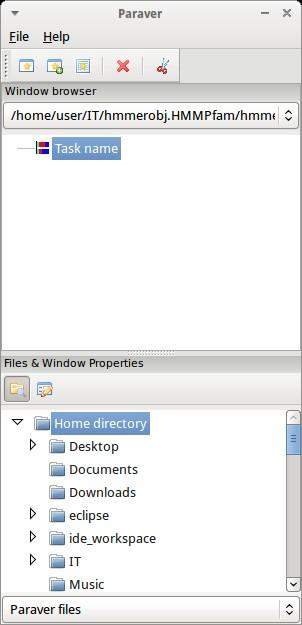
\includegraphics[width=0.45\textwidth]{./Sections/3_Visualization/Figures/1.jpeg}
    \caption{Paraver menu}
    \label{fig:trace_1}
\end{figure}

\begin{figure}[ht!]
  \centering
    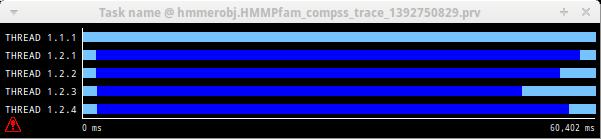
\includegraphics[width=1.0\textwidth]{./Sections/3_Visualization/Figures/2.jpeg}
    \caption{Trace file}
    \label{fig:trace_2}
\end{figure}

\subsection{View Adjustment}

In a Paraver view, a red exclamation sign may appear in the bottom-left corner (see Figure \ref{fig:trace_2} in the previous section). This means that some event values are not being shown (because they are out of the current view scope), so little adjustments must be made to
view the trace correctly:

\begin{itemize}
 \item Fit window: modifies the view scope to fit and display all the events in the current window.
	\begin{itemize}
	    \item Right click on the trace window
	    \item Choose the option Fit Semantic Scale / Fit Both
	\end{itemize}
\end{itemize}

\begin{figure}[ht!]
  \centering
    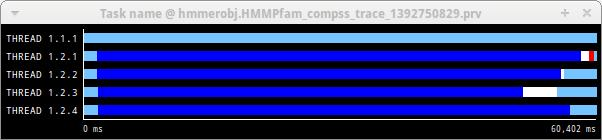
\includegraphics[width=1.0\textwidth]{./Sections/3_Visualization/Figures/3.jpeg}
    \caption{Paraver view adjustment: Fit window}
\end{figure}

\begin{itemize} 
 \item View Event Flags: marks with a green flag all the emitted the events.
	\begin{itemize}
	    \item Right click on the trace window
	    \item Chose the option View / Event Flags
	\end{itemize}
\end{itemize}
 
\begin{figure}[ht!]
  \centering
    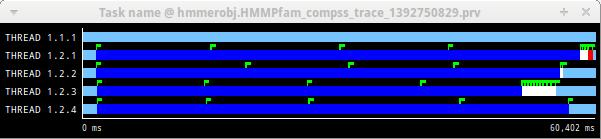
\includegraphics[width=1.0\textwidth]{./Sections/3_Visualization/Figures/4.jpeg}
    \caption{Paraver view adjustment: View Event Flags}
\end{figure}

\begin{itemize}
 \item Show Info Panel: display the information panel. In the tab ``Colors'' we can see the legend of the colors shown in the view.
	\begin{itemize}
	    \item Right click on the trace window
	    \item Check the Info Panel option
	    \item Select the Colors tab in the panel
	\end{itemize}
\end{itemize}

\begin{figure}[ht!]
  \centering
    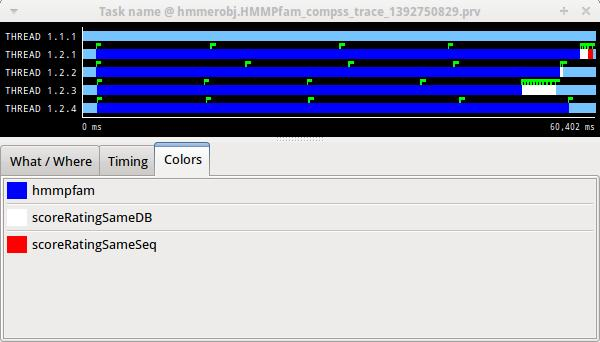
\includegraphics[width=1.0\textwidth]{./Sections/3_Visualization/Figures/5.jpeg}
    \caption{Paraver view adjustment: Show info panel}
\end{figure}

\begin{itemize}
 \item Zoom: explore the tracefile more in-depth by zooming into the most relevant sections.
	\begin{itemize}
	    \item Select a region in the trace window to see that region in detail
	    \item Repeat the previous step as many times as needed
	    \item The undo-zoom option is in the right click panel
	\end{itemize}
\end{itemize}

\begin{figure}[ht!]
  \centering
    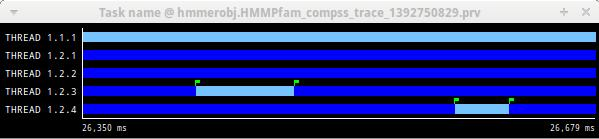
\includegraphics[width=1.0\textwidth]{./Sections/3_Visualization/Figures/6.jpeg}
    \caption{Paraver view adjustment: Zoom configuration}
\end{figure}

\begin{figure}[ht!]
  \centering
    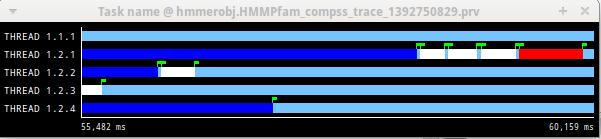
\includegraphics[width=1.0\textwidth]{./Sections/3_Visualization/Figures/6_2.jpeg}
    \caption{Paraver view adjustment: Zoom configuration}
\end{figure}
